\chapter{Figures and Plots}

This chapter collects all relevant figures that illustrate the
geometric structures of the spiral, the cone, and the helix.

\section{2D Spiral}
\begin{figure}[H]
\centering
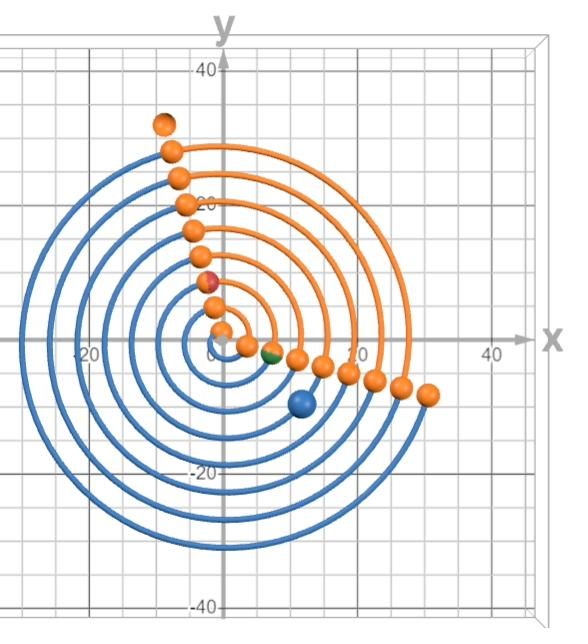
\includegraphics[width=0.8\textwidth]{bilder/spirale}
\caption{Archimedean spiral $r(\theta)=\frac{6}{\pi^2}\theta$ with
    the integer points of the sequence $k(n)$ marked.
    The green-orange point corresponds to $n=11$, the red-orange
    point to $n=13$. The blue point is a freely placeable
    reference point on the spiral path.}
\end{figure}

\section{3D Conical Helix}
\begin{figure}[H]
\centering
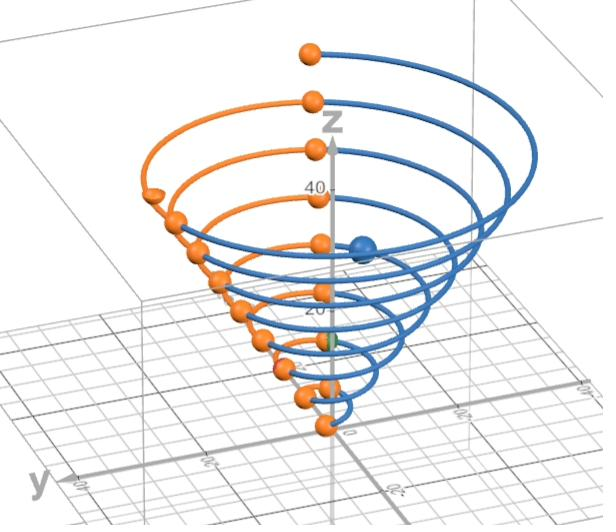
\includegraphics[width=0.8\textwidth]{bilder/kegelhelix}
\caption{Conical helix $\gamma(\theta)$ in three-dimensional space; primes
    $p>3$ appear as highlighted discrete points. The orange-coloured
    arc segments represent the arc length over the minor steps
    ($\Delta n = 2$), while the blue-coloured arc segments represent the arc length
    over the major steps ($\Delta n = 4$).}
\label{fig:kegelhelix1}
\end{figure}


\begin{figure}
    \centering
    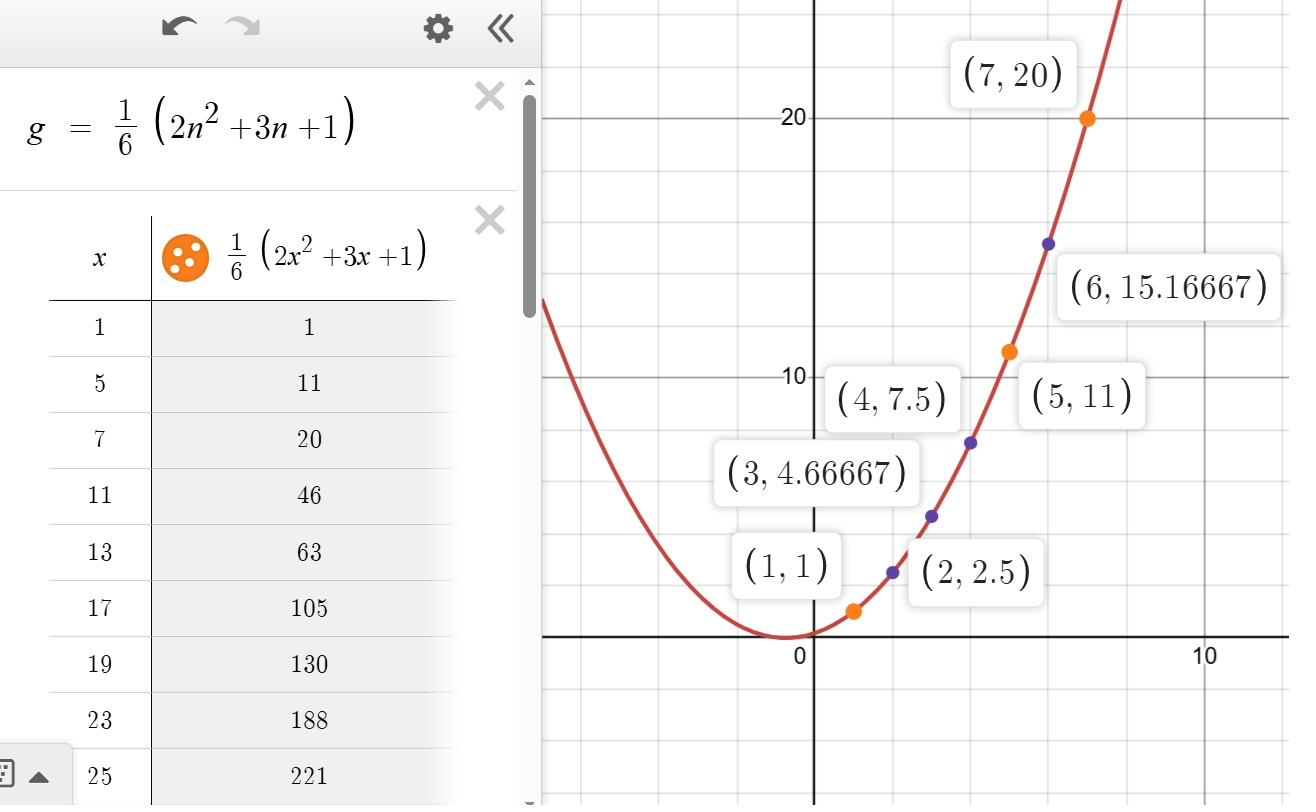
\includegraphics[width=0.5\linewidth]{bilder/Quadratische_kurve1}
    \caption{Parabolic curve $k(n)=\frac{1}{6}(2n^2+3n+1)$ with integer points at $n\equiv1,5\pmod{6}$}
    \label{fig:quadratischekurve1}
\end{figure}

\begin{figure}
    \centering
    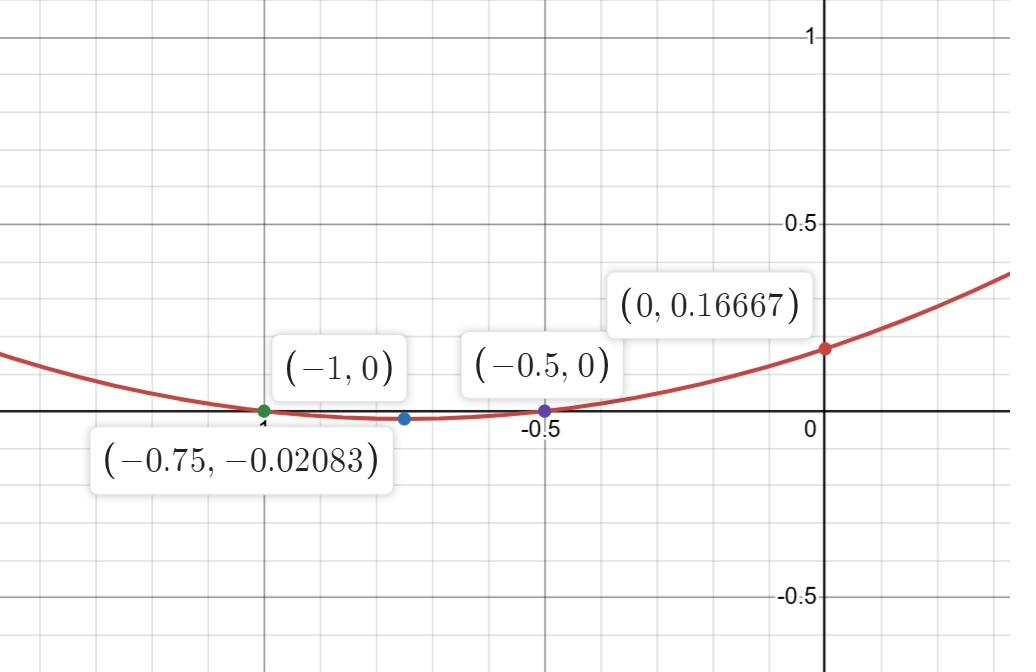
\includegraphics[width=0.5\linewidth]{bilder/Quadratische_kurve2}
    \caption{Zeros of the function $k(n)$: $n_1=-\frac{1}{2}$ and $n_2=-1$, together with the $y$-intercept and the vertex of the curve.}
    \label{fig:quadratischekurve2}
\end{figure}

\begin{figure}
    \centering
    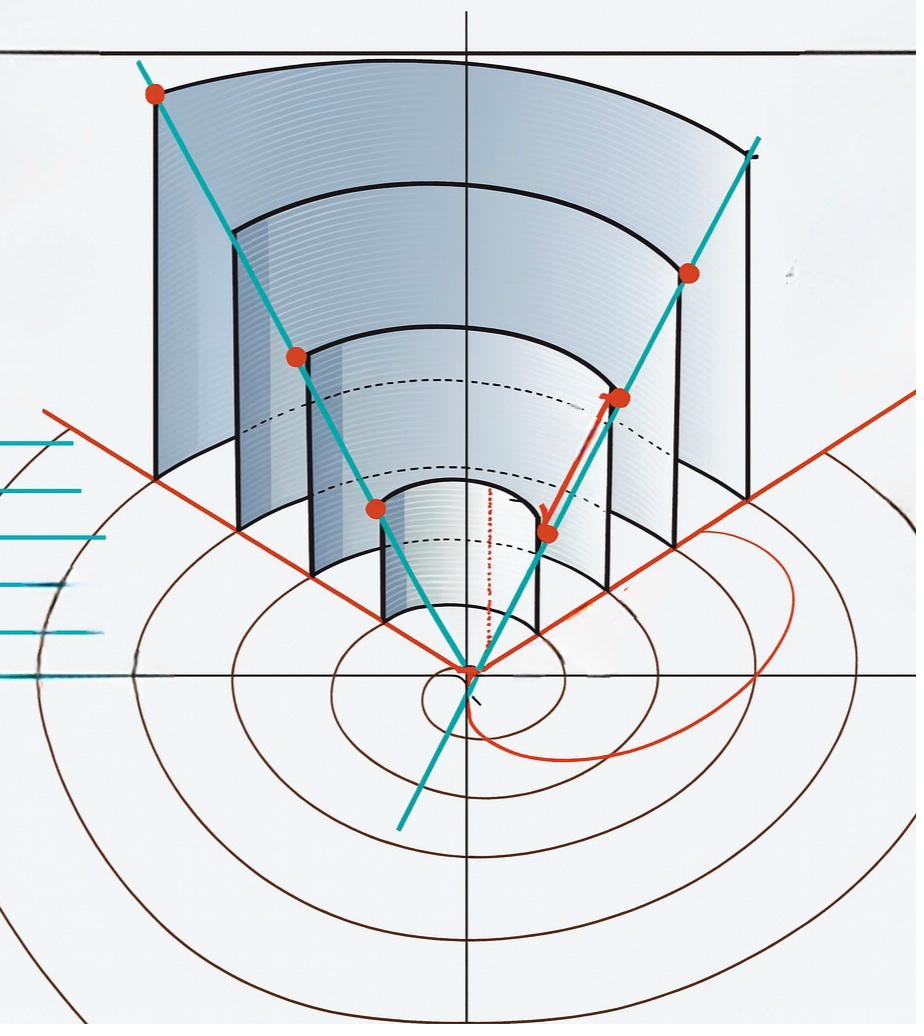
\includegraphics[width=0.5\linewidth]{bilder/image_1770054184004}
    \caption{Curve segments of the minor steps ($\Delta n=2$) on the
    parabolic curve (twin zones). The major segments have been
    omitted for clarity.}
    \label{fig:minorsegments1}
\end{figure}
